\begin{figure}
	\centering
	\begin{subfigure}[b]{0.3\textwidth}
		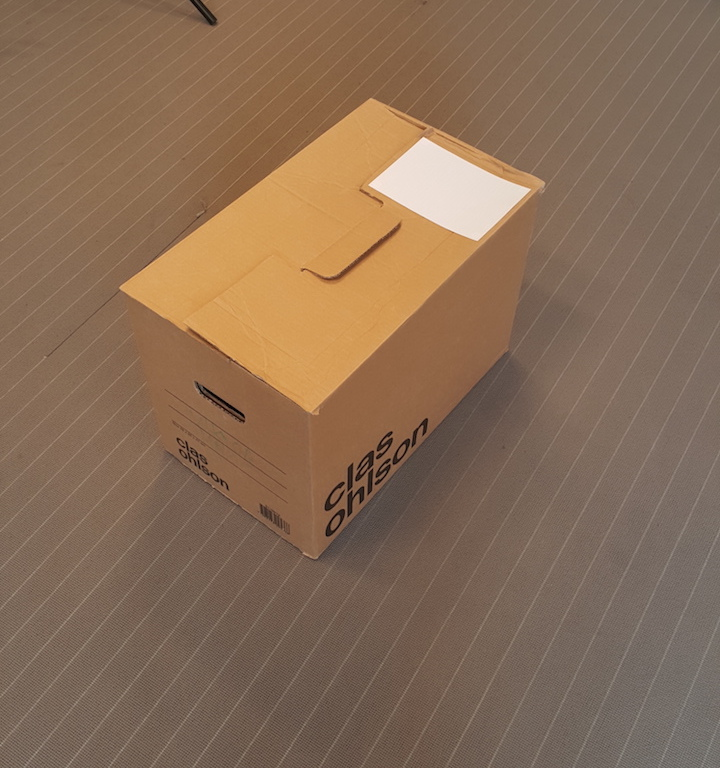
\includegraphics[width=\textwidth]{figures/package_1.jpg}
		\caption{}
		\label{fig:package_1}
	\end{subfigure}%
	~~~ %add desired spacing between images, e. g. ~, \quad, \qquad, \hfill etc.
	%(or a blank line to force the subfigure onto a new line)
	\begin{subfigure}[b]{0.3\textwidth}
		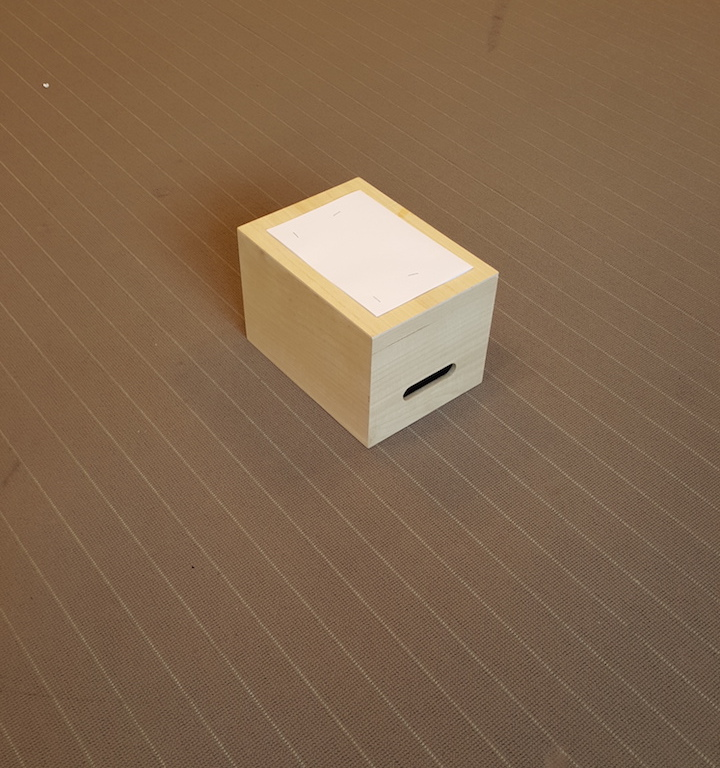
\includegraphics[width=\textwidth]{figures/package_2.jpg}
		\caption{}
		\label{fig:package_2}
	\end{subfigure}
	\vspace{3mm}\\
	\begin{subfigure}[b]{0.3\textwidth}
		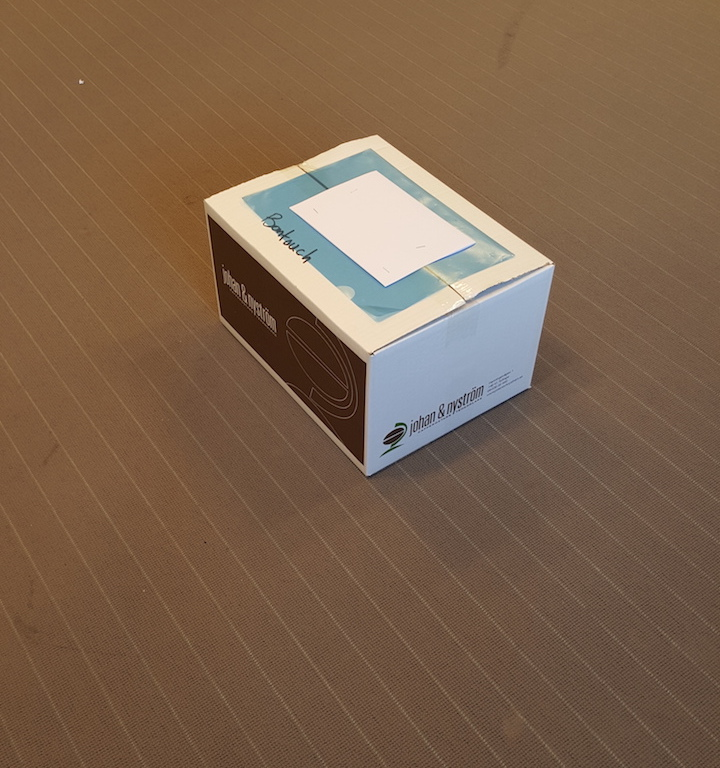
\includegraphics[width=\textwidth]{figures/package_3.jpg}
		\caption{}
		\label{fig:package_3}
	\end{subfigure}
	~~~
	\begin{subfigure}[b]{0.3\textwidth}
		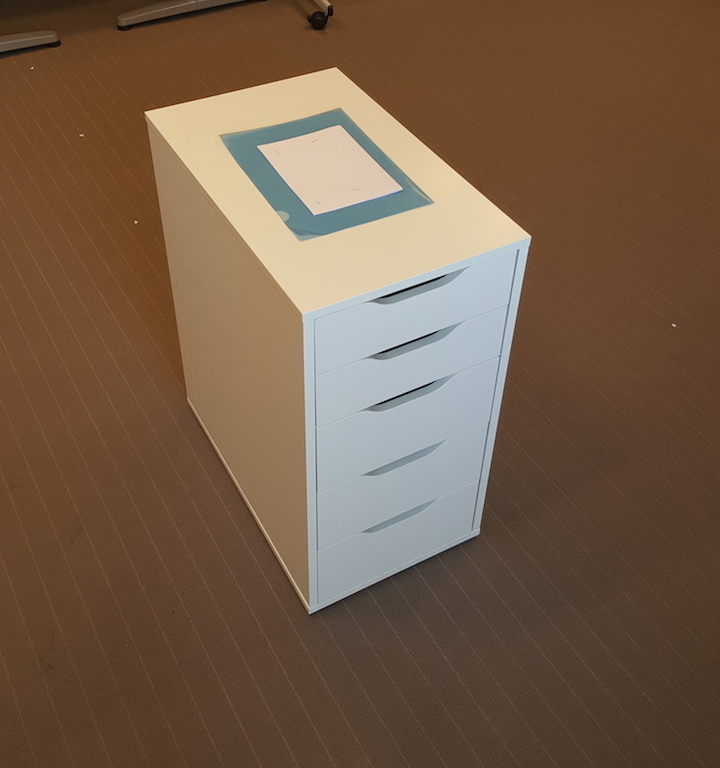
\includegraphics[width=\textwidth]{figures/package_4.jpg}
		\caption{}
		\label{fig:package_4}
	\end{subfigure}
	\vspace{3mm}\\
	\begin{subfigure}[b]{0.3\textwidth}
		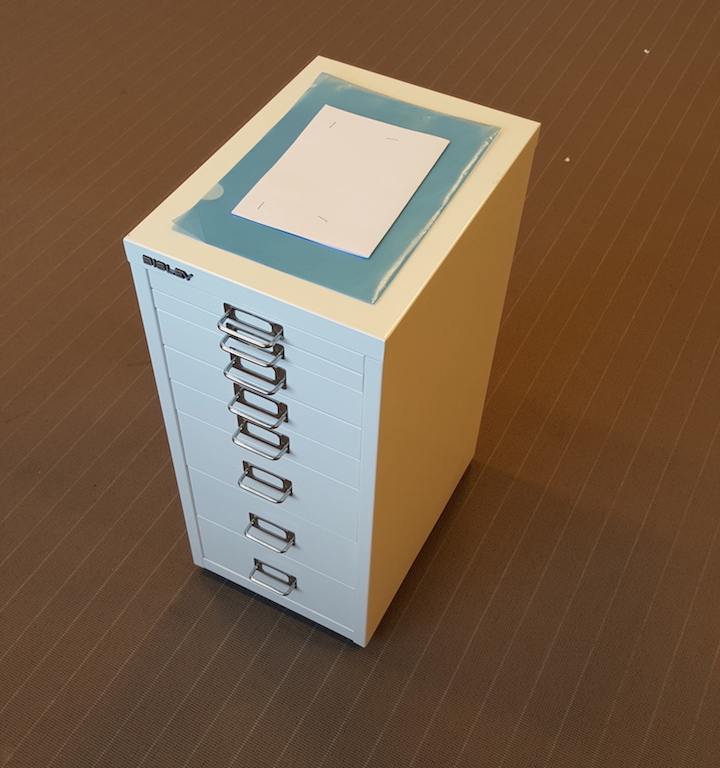
\includegraphics[width=\textwidth]{figures/package_5.jpg}
		\caption{}
		\label{fig:package_5}
	\end{subfigure}
	\caption{The packages in the test dataset. (a) Package 1: A moving box ($580 \times 350 \times 405$ mm). (b) Package 2: A small wooden box ($260 \times 191 \times 177$ mm). (c) Package 3: A lightly textured cardboard box ($385 \times 295 \times 225$ mm). (d) Package 4: A white wooden filing cabinet ($580 \times 360 \times 690$ mm). (e) Package 5: A white metal filing cabinet ($383 \times 280 \times 605$ mm).}\label{fig:packages}
\end{figure}